\documentclass{article}

\usepackage[final]{neurips_2024}

\usepackage[utf8]{inputenc}
\usepackage[T1]{fontenc}
\usepackage{hyperref}
\usepackage{url}
\usepackage{booktabs}
\usepackage{amsmath}
\usepackage{amsfonts}
\usepackage{amssymb}
\usepackage{microtype}
\usepackage{xcolor}
\usepackage{graphicx}
\usepackage{tikz}
\usetikzlibrary{arrows.meta, positioning, fit}
\usepackage{enumitem}
\setlist{leftmargin=*,noitemsep,topsep=2pt,parsep=0pt}

% AUTO-GENERATED by scripts/08_make_report_numbers.py -- do not edit
\newcommand{\NTrain}{6251}
\newcommand{\NDev}{883}
\newcommand{\NTest}{1147}
\newcommand{\NTotal}{8281}
\newcommand{\FactsPerDoc}{30.7}
\newcommand{\TokensPerDoc}{839}
\newcommand{\PctModTableTest}{62}
\newcommand{\PctModTextTest}{25}
\newcommand{\PctModHybridTest}{14}
\newcommand{\PctStepsOneTest}{57}
\newcommand{\PctStepsTwoTest}{36}
\newcommand{\PctStepsThreePlusTest}{7}
\newcommand{\PctRatioTest}{69}
\newcommand{\DslOk}{8281}
\newcommand{\DslTotal}{8281}
\newcommand{\SerTotal}{9901}
\newcommand{\SerExactPct}{92.5}
\newcommand{\SerWsPct}{7.0}
\newcommand{\SerHeaderPct}{0.6}
\newcommand{\SerOther}{0}
\newcommand{\OperandCovAll}{99.9}
\newcommand{\ProgCovAll}{99.7}
\newcommand{\GroundedTest}{95.5}
\newcommand{\RelFull}{86.5}
\newcommand{\RelFact}{89.8}
\newcommand{\RelChance}{11.5}
\newcommand{\RelTable}{95.3}
\newcommand{\RelFactTable}{96.2}
\newcommand{\RelText}{84.1}
\newcommand{\RelFactText}{85.2}
\newcommand{\RelHybrid}{51.3}
\newcommand{\RelFactHybrid}{77.2}
\newcommand{\NFailTotal}{155}
\newcommand{\NFailTable}{33}
\newcommand{\FailShareTable}{21}
\newcommand{\QShareTable}{62}
\newcommand{\NFailText}{45}
\newcommand{\FailShareText}{29}
\newcommand{\QShareText}{25}
\newcommand{\NFailHybrid}{77}
\newcommand{\FailShareHybrid}{50}
\newcommand{\QShareHybrid}{14}
\newcommand{\RelAtTwoAll}{72.4}
\newcommand{\RelAtThreeAll}{79.9}
\newcommand{\NIncomplete}{155}
\newcommand{\NIncompleteGrounded}{106}
\newcommand{\PctIncompleteGrounded}{68}
\newcommand{\RelTestEA}{60.5}
\newcommand{\RelTestPA}{58.8}
\newcommand{\RelOracleEA}{60.6}
\newcommand{\RelOraclePA}{58.9}
\newcommand{\MineTestEA}{60.1}
\newcommand{\MineTestPA}{58.2}
\newcommand{\MineOracleEA}{60.2}
\newcommand{\MineFull}{86.1}
\newcommand{\MineFactRecall}{89.2}
\newcommand{\MineHybrid}{57.0}
\newcommand{\MineTable}{93.5}
\newcommand{\MineText}{84.1}
\newcommand{\NWrong}{453}
\newcommand{\NGenOnly}{356}
\newcommand{\NBoth}{89}
\newcommand{\NRetOnly}{8}
\newcommand{\PctGenOnly}{78.6}
\newcommand{\PctBoth}{19.6}
\newcommand{\PctRetOnly}{1.8}
\newcommand{\EAThreePlus}{21.4}
\newcommand{\EAOneStep}{66.8}
\newcommand{\EAHybrid}{44.9}
\newcommand{\EATable}{68.1}
\newcommand{\NCompleteWrong}{356}
\newcommand{\NStructCompl}{203}
\newcommand{\NOperandCompl}{152}

% AUTO-GENERATED by scripts/12_phase2_analysis.py
\newcommand{\SingleEAMean}{60.6}
\newcommand{\SingleEASd}{0.7}
\newcommand{\SinglePAMean}{58.7}
\newcommand{\SinglePASd}{0.6}
\newcommand{\SingleEAMin}{59.6}
\newcommand{\SingleEAMax}{61.1}
\newcommand{\NRuns}{4}
\newcommand{\VoteThree}{62.4}
\newcommand{\VoteFour}{63.0}
\newcommand{\AnyThree}{68.9}
\newcommand{\AnyFour}{71.5}
\newcommand{\MechUnparsable}{0.0}
\newcommand{\MechTooFewSteps}{23.7}
\newcommand{\MechTooManySteps}{18.6}
\newcommand{\MechWrongOperator}{14.4}
\newcommand{\MechArgsSwapped}{2.3}
\newcommand{\MechWrongConstant}{3.7}
\newcommand{\MechWrongReference}{1.1}
\newcommand{\MechWrongOperand}{36.2}
\newcommand{\MechFewManyShare}{42.3}
\newcommand{\NWrongPooled}{1809}
\newcommand{\BeamTopEA}{61.5}
\newcommand{\BeamTopPA}{59.5}
\newcommand{\GreedyBeamRunEA}{61.1}
\newcommand{\MargEA}{61.9}
\newcommand{\MargPA}{59.8}
\newcommand{\LearnEA}{62.1}
\newcommand{\LearnPA}{60.0}
\newcommand{\MargK}{8}
\newcommand{\MargT}{2.0}
\newcommand{\LearnModel}{gbm d3}
\newcommand{\LearnFixed}{11}
\newcommand{\LearnBroke}{4}
\newcommand{\LearnCIlo}{0.0}
\newcommand{\LearnCIhi}{1.3}
\newcommand{\MargFixed}{6}
\newcommand{\MargBroke}{1}
\newcommand{\MargP}{0.12}
\newcommand{\OracleKOne}{61.5}
\newcommand{\OracleKTwo}{69.3}
\newcommand{\OracleKFour}{73.8}
\newcommand{\OracleKEight}{77.0}
\newcommand{\OracleKSixteen}{80.3}
\newcommand{\ThreePlusBase}{26.2}
\newcommand{\ThreePlusRerank}{29.8}
\newcommand{\ThreePlusLearn}{29.8}
\newcommand{\NThreePlus}{84}


\newcommand{\todo}[1]{\textcolor{red}{[\textbf{TODO:} #1]}}
\newcommand{\code}[1]{\texttt{#1}}

\title{Diagnosing and Repairing Multi-Step Reasoning Failures in Numerical Question Answering over Financial Reports: Final Report}

\author{
  Sameeksha Keshav \\
  Dept.\ of Computer Science Engineering \\
  North Carolina State University \\
  \texttt{skeshav2@ncsu.edu}
}

\begin{document}

\maketitle

\begin{abstract}
I study why retriever--generator models fail at numerical question answering over financial reports (FinQA), and test one repair. I reimplemented a FinQANet-style retriever and pointer generator from scratch together with a DSL interpreter validated on all \NTotal{} questions, and built a multi-axis error taxonomy. Over \NRuns{} training runs with \code{roberta-base} the generator reaches \SingleEAMean\,$\pm$\,\SingleEASd\% test execution accuracy (published: 61.2 with RoBERTa-large). The taxonomy shows that retrieval is imperfect, particularly for hybrid table-and-text questions, but is not the bottleneck: giving the generator the gold evidence changes test accuracy by under 0.5 points. The errors are in the generated program: 71\% of the failures on programs with 3+ steps are programs that stop too early, and on one-step questions wrong document operands and over-long programs dominate. As a targeted repair I added beam search with execution-guided reranking. The correct answer is among the top 16 beams for \OracleKSixteen\% of test questions, yet reranking recovers only \MargEA--\LearnEA\% against \BeamTopEA\% for beam top-1; the gain is small and not statistically significant. Voting across independently trained models helps more (\VoteThree\% with three models), which indicates that a single model's candidates share systematic errors. I did not carry out the planned MultiHiertt check. Code: \todo{GitHub link}.
\end{abstract}

\section{Introduction}

\paragraph{Background.} Analysts answer quantitative questions from filings (``what was the change in operating margin?'') by finding numbers scattered over tables and prose and combining them with the right arithmetic. FinQA \citep{chen2021finqa} turns this into a benchmark: given an earnings report, produce an executable \emph{program} over the evidence whose result is the answer.

\paragraph{Existing approaches.} The FinQA paper introduced FinQANet, a two-stage \emph{retriever--generator}: a cross-encoder selects the supporting facts, and a decoder writes the program, copying numbers from them. Later work keeps this design and improves its parts: DyRRen \citep{li2023dyrren} re-ranks the retrieved facts at each generation step, and APOLLO \citep{sun2022apollo} changes the training objectives of retriever and generator. I restrict this project to this family of non-LLM models, which is small enough to retrain and instrument fully.

\paragraph{Limitations.} These systems are compared by aggregate accuracy. A wrong answer can come from missing evidence, a wrong operator structure, a wrong operand or an arithmetic slip, and each calls for a different fix, but published work does not say which of them dominates, so it is unclear which component an improvement should target.

\paragraph{Challenges.} Failures of the two stages are entangled: a program can be wrong because evidence was missed or despite complete evidence, and separating the cases needs a controlled counterfactual. Programs are also hard to compare, since several programs can be correct (commutative operands, independent steps, a constant versus an equal copied number) and an operand value can occur in several cells. Finally, reported differences of a point or less are of the same size as the variation between training runs, so every claim needs a variance estimate.

\paragraph{Approach.} I reimplement a FinQANet-style retriever and pointer generator from scratch, together with a program interpreter and metrics validated on all gold programs; build a multi-axis error taxonomy whose failure locus comes from an oracle-evidence counterfactual; classify why wrong programs are wrong; and test one repair suggested by the findings, beam search with execution-guided reranking.

\paragraph{Contributions.}
\begin{itemize}
  \item A from-scratch retriever--generator baseline and DSL interpreter (all \DslOk{} of \DslTotal{} gold programs re-execute to the stored answer), reaching \SingleEAMean\,$\pm$\,\SingleEASd\% test EA over \NRuns{} runs with \code{roberta-base}.
  \item A multi-axis error taxonomy with an oracle-evidence locus. Its main finding: retrieval is imperfect (hybrid questions are \QShareHybrid\% of the test set but \FailShareHybrid\% of top-5 retrieval failures) but is not the bottleneck, since gold evidence changes test EA by under 0.5 points.
  \item A mechanism-level analysis of wrong programs: for 3+ step programs 71\% of errors are programs that stop too early; for one-step programs wrong operands and overlong programs dominate.
  \item A repair study. The correct answer is among the top 16 beams for \OracleKSixteen\% of questions, but beam reranking recovers only 0.4--0.6 EA points (not significant); voting across independently trained models gains \VoteThree\%. This is reported as a negative result with its limits.
  \item Open code, scripts and tests to regenerate every table in this report.
\end{itemize}

\section{Method}
\subsection{Dataset and processing}

\paragraph{Data.} FinQA contains \NTotal{} expert-written questions over S\&P~500 earnings reports, split \NTrain/\NDev/\NTest{} (train/dev/test). A document has pre-text sentences, one table and post-text sentences, on average \FactsPerDoc{} facts and about \TokensPerDoc{} tokens. Each question has a gold program in a ten-operation DSL (\code{add}, \code{subtract}, \code{multiply}, \code{divide}, \code{exp}, \code{greater}, \code{table\_max/min/sum/average}) and gold supporting facts. Table~\ref{tab:data} gives split statistics; Figure~\ref{fig:axes} shows the distribution over the diagnostic axes used later.

\begin{table}[h]
\centering\small
\begin{tabular}{lrrrrrrrrr}
\toprule
 & & & & \multicolumn{3}{c}{\% by program steps} & \multicolumn{3}{c}{\% by gold evidence} \\
\cmidrule(lr){5-7}\cmidrule(lr){8-10}
Split & Questions & Facts/doc & Tokens/doc & 1 & 2 & 3+ & table & text & hybrid \\
\midrule
Train & 6,251 & 30.6 & 841 & 59 & 32 & 8 & 63 & 23 & 14 \\
Dev & 883 & 30.4 & 834 & 59 & 33 & 8 & 61 & 22 & 16 \\
Test & 1,147 & 31.3 & 826 & 57 & 36 & 7 & 62 & 25 & 14 \\
\bottomrule
\end{tabular}

\caption{FinQA statistics computed by \code{scripts/03\_dataset\_stats.py}. ``Hybrid'' means the gold evidence uses both table rows and text sentences.}\label{tab:data}
\end{table}

\begin{figure}[h]
\centering
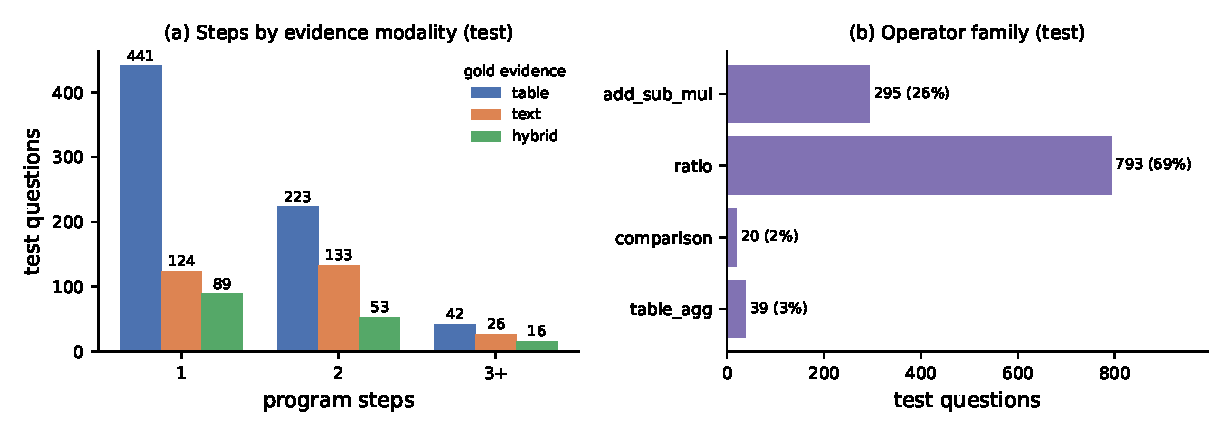
\includegraphics[width=\textwidth]{figures/dataset_axes.pdf}
\caption{Distribution of questions over the gold-derived axes (program length, evidence modality, operator family).}\label{fig:axes}
\end{figure}

\paragraph{Processing.} All code is my own; only the three JSON files are taken from the public release. (i) \emph{Facts.} Pre- and post-text are concatenated into \code{text\_i}; each table row $j$ becomes \code{table\_j}, with row~0 the header. (ii) \emph{Label-free serialization.} A row is rendered as ``the $\langle$label$\rangle$ of $\langle$column$\rangle$ is $\langle$value$\rangle$'' for every column, in a fixed format that does not depend on whether the row is gold. The upstream README documents an earlier leak where gold rows were formatted differently from negatives; I avoid this by construction and compare my output with the dataset's stored gold-row text: of \SerTotal{} gold table rows, \SerExactPct\% match exactly, \SerWsPct\% differ only in whitespace, \SerHeaderPct\% are header rows that differ in format, and \SerOther{} differ in content. (iii) \emph{Program interpreter.} I wrote a depth-aware parser and an executor for the DSL. Executing every gold program reproduces the stored answer in \DslOk{} of \DslTotal{} cases. Getting there required handling cells such as ``22\% ( 22 \% )'', duplicate row labels (the last one wins) and comparison after rounding to five decimals. (iv) \emph{Operand grounding.} The generator copies numbers rather than inventing them, so I extract number and row-label candidates with character offsets. Over all questions \OperandCovAll\% of gold operands are copyable from the full document, and \ProgCovAll\% of programs have every operand available. (v) \emph{Dataset quirks.} One gold id (\code{text\_-1}) points to a non-existent fact and is dropped. Several questions have duplicate-valued operands, which is why training uses a marginal loss over duplicates (Sec.~\ref{sec:model}).

\subsection{Model design and metrics}\label{sec:model}

\begin{figure}[h]
\centering
\resizebox{\textwidth}{!}{%
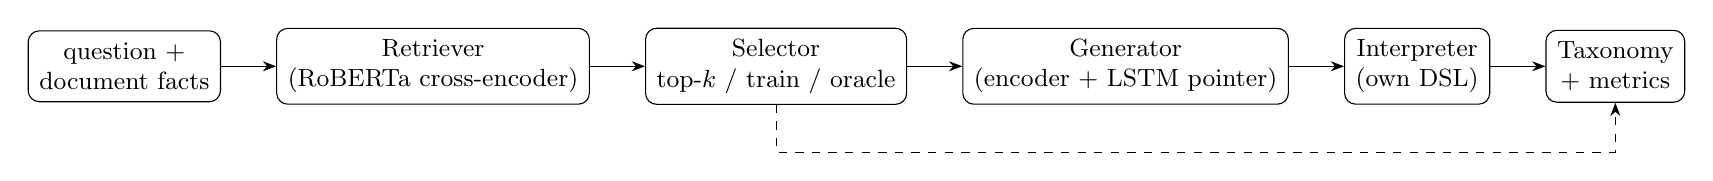
\begin{tikzpicture}[node distance=7mm, box/.style={draw, rounded corners, align=center, minimum height=9mm, inner sep=4pt, font=\small}, >=Stealth]
\node[box] (q) {question +\\document facts};
\node[box, right=of q] (ret) {Retriever\\(RoBERTa cross-encoder)};
\node[box, right=of ret] (sel) {Selector\\top-$k$ / train / oracle};
\node[box, right=of sel] (gen) {Generator\\(encoder + LSTM pointer)};
\node[box, right=of gen] (exe) {Interpreter\\(own DSL)};
\node[box, right=of exe] (tax) {Taxonomy\\+ metrics};
\draw[->] (q)--(ret); \draw[->] (ret)--(sel); \draw[->] (sel)--(gen); \draw[->] (gen)--(exe); \draw[->] (exe)--(tax);
\draw[->, dashed] (sel.south) -- ++(0,-6mm) -| (tax.south);
\end{tikzpicture}}
\caption{Pipeline. The dashed edge carries the selected evidence into the taxonomy so retrieval and generation errors can be separated.}\label{fig:pipe}
\end{figure}

\paragraph{Retriever.} Following FinQANet \citep{chen2021finqa}, a cross-encoder reads (question, fact) and outputs a relevance score $s(q,f)=\sigma(\mathbf{w}^\top h_{\textsc{cls}}(q,f))$ with RoBERTa \citep{liu2019roberta} as the encoder, trained with binary cross-entropy over gold facts and sampled negatives. The selector then takes the top $k$ facts. For training the generator I also use \emph{train} (top-$k$ $\cup$ gold) and \emph{oracle} (gold plus the best non-gold up to $k$) selectors, all in a fixed label-free fact order.

\paragraph{Generator.} The selected facts are encoded together with the question. A program is generated token by token by an LSTM decoder with attention. At step $t$ the output distribution is one softmax over reserved tokens (operators, parentheses, constants, step references \code{\#0}--\code{\#7}, end) \emph{and} copy candidates (numbers and row labels in the input):
\begin{equation}
p(y_t \mid y_{<t}) = \mathrm{softmax}\big([\,W_r d_t \,;\, \{ e_c^\top W_c d_t \}_{c\in\mathcal{C}}\,]\big),
\end{equation}
where $d_t$ is the decoder state, $e_c$ the encoder representation of candidate $c$ and $\mathcal{C}$ the candidate set. When several candidates share the gold value, the loss marginalizes over them: $\mathcal{L}=-\sum_t \log \sum_{c\in G_t} p(c\mid y_{<t})$, with $G_t$ the set of correct tokens at step $t$.

\paragraph{Beam search and execution-guided reranking.} For the repair I decode with beam search (up to 16 finished programs per question, ranked by summed log-probability) and choose among the candidates by their \emph{executed answers}. \emph{Voting}: programs that execute to the same answer pool their probability mass $\exp\big((\log p-\max\log p)/T\big)$, the answer with the most mass wins and its most probable program is returned; the beam size $k$ and temperature $T$ are chosen on dev. \emph{Learned}: a classifier (logistic regression or gradient boosting, chosen by 5-fold cross-validation on dev) scores each candidate from 38 features (log-probability and rank, vote share and number of distinct answers, program length and shape, answer plausibility, question cues); it is trained on the dev beams, since the generator never trained on dev, and applied once to test. In both cases the answer is chosen by the reranker and the program by the generator's probability, so program accuracy is not degraded when several programs give the same answer.

\paragraph{Metrics.} \emph{Execution accuracy} (EA) compares the executed answer with the gold answer after rounding to five decimals. \emph{Program accuracy} (PA) compares a canonical form of the program: commutative operands are sorted, independent steps are order-normalized, and a constant is treated as equal to a copied number of the same value. This last choice is lenient and is documented and tested; for example \code{divide(637, const\_5)} equals \code{divide(637, 5)} under PA. The published FinQANet numbers are 61.24 EA and 58.86 PA with RoBERTa-large \citep{chen2021finqa}.

\paragraph{Error taxonomy.} Every test question is tagged on gold-derived axes (steps 1/2/3+, modality table/text/hybrid, operator family, number of gold facts) and, once predictions exist, on prediction-derived axes: \emph{retrieval status} (complete, partial, miss), \emph{operands grounded}, \emph{error type} (non-executable, structure error, operand error, found by comparing predicted and gold \emph{skeletons} with operands masked), and \emph{locus}. The locus uses a counterfactual: rerun the generator with the oracle selector; if the answer becomes correct the error was in retrieval, if it stays wrong it was in generation, and if neither selector is correct it is recorded as both.

\section{Results}

\paragraph{Where the released retriever loses evidence.} The FinQA authors released the retriever's ranked facts. I analyse these test-set rankings with my own taxonomy code, with one caveat: I do not know the exact checkpoint that produced them, so this is an analysis of released outputs, not a reproduction. \emph{Full recall@5} is the share of questions whose entire gold evidence is in the top~5. It is \RelFull\% overall, against \RelChance\% for a random top-5. Table~\ref{tab:ret} and Figure~\ref{fig:ret} break this down. Table-only questions are retrieved well (\RelTable\%), text-only less so (\RelText\%), and hybrid questions poorly (\RelHybrid\% full recall, although \RelFactHybrid\% of their individual gold facts are found). Hybrid questions are \QShareHybrid\% of the test set but account for \NFailHybrid{} of the \NFailTotal{} top-5 failures (\FailShareHybrid\%). Program length matters much less than evidence modality: recall is 87.3\% for one-step and 84.5\% for 3+ step programs.

\begin{table}[h]
\centering\small
\begin{tabular}{lrrr}
\toprule
Category (test) & $n$ & Full recall@5 & Fact recall@5 \\
\midrule
All questions & 1147 & 86.5 & 89.8 \\
\midrule
\multicolumn{4}{l}{\emph{Gold evidence modality}} \\
\quad table & 706 & 95.3 & 96.2 \\
\quad text & 283 & 84.1 & 85.2 \\
\quad hybrid & 158 & 51.3 & 77.2 \\
\multicolumn{4}{l}{\emph{Program steps}} \\
\quad 1 & 654 & 87.3 & 90.9 \\
\quad 2 & 409 & 85.6 & 87.6 \\
\quad 3+ & 84 & 84.5 & 89.8 \\
\multicolumn{4}{l}{\emph{Operator family}} \\
\quad add\_sub\_mul & 295 & 83.1 & 87.5 \\
\quad ratio & 793 & 86.9 & 90.1 \\
\quad comparison & 20 & 95.0 & 97.2 \\
\quad table\_agg & 39 & 100.0 & 100.0 \\
\midrule
Random top-5 (chance) & & 11.5 & \\
\bottomrule
\end{tabular}

\caption{Released-retriever top-5 evidence recall on the test set, by taxonomy axis (\code{scripts/02\_retrieval\_analysis.py}).}\label{tab:ret}
\end{table}

\begin{figure}[h]
\centering
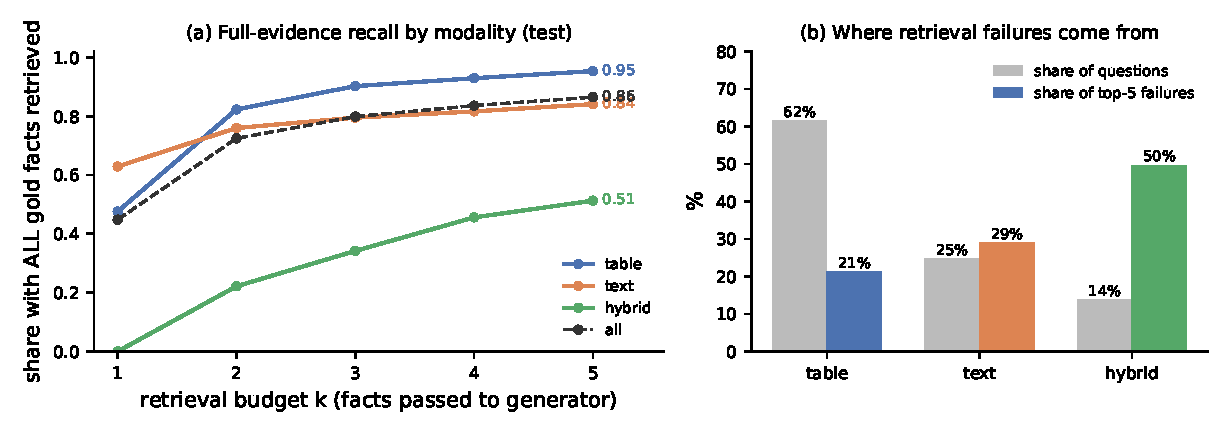
\includegraphics[width=0.8\textwidth]{figures/retrieval_released.pdf}
\caption{Full evidence recall as the cut-off $k$ grows, split by modality (\code{scripts/04\_plot\_retrieval.py}).}\label{fig:ret}
\end{figure}

\paragraph{Missing evidence is not always fatal.} Of the \NIncomplete{} test questions whose top-5 misses part of the gold evidence, \NIncompleteGrounded{} (\PctIncompleteGrounded\%) still have all operands copyable from the retrieved facts. Whether the generator then produces the right program is what the oracle counterfactual below measures.

\paragraph{Trained baseline.} I trained both models on a Kaggle T4 with \code{roberta-base} (not RoBERTa-large as in the published number, so some gap is expected); the checkpoint is chosen by dev EA. The table~\ref{tab:base} runs use seed~0; to estimate run-to-run variation I trained the released-retrieval generator \NRuns{} times (seeds 0, 1, 2 and a repeat of seed 0; GPU training is not bit-reproducible): test EA \SingleEAMean\,$\pm$\,\SingleEASd\% (range \SingleEAMin--\SingleEAMax), PA \SinglePAMean\,$\pm$\,\SinglePASd\%. My retriever reaches \MineFull\% full recall@5 on the test set (released: \RelFull\%), with \MineTable\% on table, \MineText\% on text and \MineHybrid\% on hybrid questions (released: \RelTable, \RelText, \RelHybrid). Table~\ref{tab:base} gives generator accuracy. With the released retrieval the generator reaches \RelTestEA\% EA and \RelTestPA\% PA on test (dev best 63.2\% EA), within a point of the published 61.24/58.86 although the encoder is smaller. My retriever gives \MineTestEA\% EA, a 0.4-point difference that is inside the run-to-run variation and the sampling noise of 1{,}147 test questions, and which I do not interpret.

\begin{table}[h]
\centering\small
\begin{tabular}{lrrrr}
\toprule
 & \multicolumn{2}{c}{Dev} & \multicolumn{2}{c}{Test} \\
\cmidrule(lr){2-3}\cmidrule(lr){4-5}
Setting & EA & PA & EA & PA \\
\midrule
Released retriever + top-5 evidence & 63.2 & 61.5 & 60.5 & 58.8 \\
Released retriever + gold evidence & 64.4 & 62.9 & 60.6 & 58.9 \\
My retriever + top-5 evidence & 63.2 & 61.0 & 60.1 & 58.2 \\
My retriever + gold evidence & 64.2 & 62.1 & 60.2 & 58.4 \\
\bottomrule
\end{tabular}

\caption{Generator accuracy (\%) with each retriever, using its top-5 facts or the gold facts (oracle). First run only; run-to-run standard deviation is about 0.7 points.}\label{tab:base}
\end{table}

\paragraph{Error taxonomy: retrieval is not the bottleneck.} Using the oracle counterfactual from Sec.~\ref{sec:model}, I split the \NWrong{} wrong test answers of the released-retrieval run by locus. \NGenOnly{} (\PctGenOnly\%) are generation errors with complete retrieval; \NBoth{} (\PctBoth\%) have incomplete retrieval but remain wrong when the generator is given the gold evidence; only \NRetOnly{} (\PctRetOnly\%) are fixed by gold evidence. Equivalently, oracle evidence moves test EA from \RelTestEA\% to \RelOracleEA\%. Within the \NCompleteWrong{} wrong answers with complete retrieval, \NStructCompl{} have a different operator structure from the gold program and \NOperandCompl{} have the right structure with a wrong operand. Table~\ref{tab:tax} shows where accuracy is lowest: programs with 3+ steps (\EAThreePlus\% EA, against \EAOneStep\% for one step, with almost all errors structural) and non-table evidence (hybrid \EAHybrid\%, text 50.2\%, table \EATable\%). Hybrid questions are hard for two reasons that this analysis separates: their evidence is retrieved less often, but even when it is, the generator does worse on them.

\begin{table}[h]
\centering\small
\begin{tabular}{lrrrrr}
\toprule
Category (test) & $n$ & EA & Retr.\ complete & Structure err. & Operand err. \\
\midrule
\multicolumn{6}{l}{\emph{Gold evidence}} \\
\quad table & 706 & 68.1 & 95.3 & 120 & 105 \\
\quad text & 283 & 50.2 & 84.1 & 92 & 48 \\
\quad hybrid & 158 & 44.9 & 51.3 & 57 & 30 \\
\multicolumn{6}{l}{\emph{Program steps}} \\
\quad 1 & 654 & 66.8 & 87.3 & 99 & 117 \\
\quad 2 & 409 & 58.4 & 85.6 & 109 & 61 \\
\quad 3+ & 84 & 21.4 & 84.5 & 61 & 5 \\
\bottomrule
\end{tabular}

\caption{Released-retrieval run on the test set: accuracy, share of questions with complete retrieval, and error types of wrong answers (\code{scripts/07\_taxonomy\_report.py}).}\label{tab:tax}
\end{table}

\begin{figure}[h]
\centering
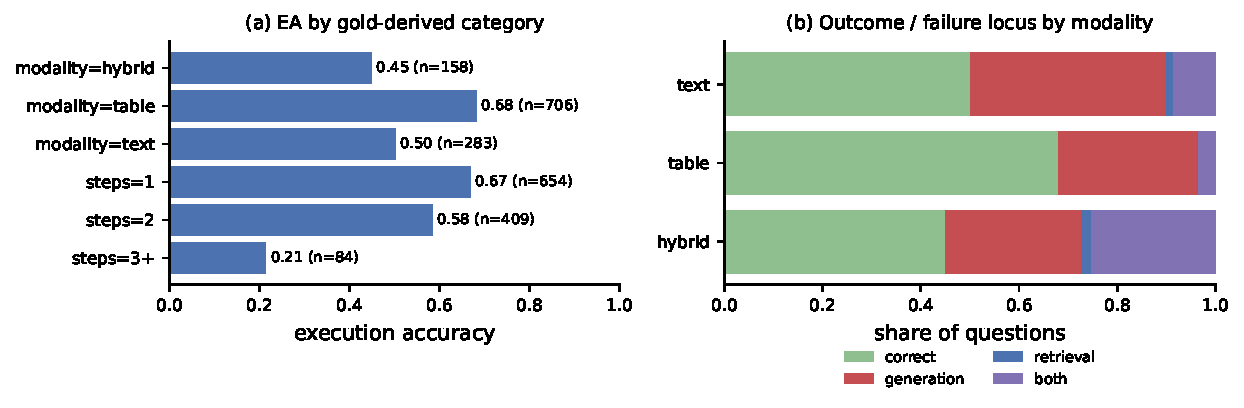
\includegraphics[width=\textwidth]{figures/taxonomy_released.pdf}
\caption{Released-retrieval run, test set: (a) EA by gold-derived category; (b) outcome and failure locus by evidence modality.}\label{fig:tax}
\end{figure}

\paragraph{How the generator fails.} The skeleton-level error types above are coarse, so I classified every wrong program by the first structural difference from the gold program (\code{mechanisms.py}), pooling the \NRuns{} runs (\NWrongPooled{} wrong answers). Table~\ref{tab:mech} shows that the mechanism depends strongly on program length. For 3+ step programs, 71\% of the errors are programs with too few steps (too few steps is \MechTooFewSteps\% of all errors), so the model stops before the program is complete. For one-step questions, wrong document operands (49\%) and programs with too many steps (29\%) dominate. Wrong operands are the largest single category overall (\MechWrongOperand\%); swapped arguments, wrong constants and wrong step references together are only 7\%. A different constant convention for percentages is not the explanation: it accounts for about 2\% of errors.

\begin{table}[h]
\centering\small
\begin{tabular}{lrrrr}
\toprule
Mechanism (\% of wrong answers) & All & 1 step & 2 steps & 3+ steps \\
\midrule
not a valid program & 0.0 & 0.0 & 0.0 & 0.0 \\
too few steps & 23.7 & 0.0 & 36.7 & 71.4 \\
too many steps & 18.6 & 29.3 & 5.7 & 15.7 \\
wrong operator (same step count) & 14.4 & 15.6 & 16.8 & 3.9 \\
arguments swapped & 2.3 & 2.7 & 2.7 & 0.0 \\
wrong constant & 3.7 & 3.2 & 4.9 & 2.4 \\
wrong step reference & 1.1 & 0.0 & 1.9 & 2.4 \\
wrong document operand & 36.2 & 49.2 & 31.3 & 4.3 \\
\midrule 
Wrong answers pooled ($n$) & 1809 & 883 & 671 & 255 \\
\bottomrule
\end{tabular}

\caption{Why wrong programs are wrong, pooled over \NRuns{} runs (test set, released retrieval), by gold program length (\code{12\_phase2\_analysis.py}). Columns do not mix: each is the distribution within its group.}\label{tab:mech}
\end{table}

\paragraph{Repair: beam search and execution-guided reranking.} The analysis suggests the generator often has the right program available but does not rank it first. Beam search tests this. Table~\ref{tab:p2} and Figure~\ref{fig:oracle} show that the right answer is among the top 16 beams for \OracleKSixteen\% of test questions (top-1: \OracleKOne\%, top-4: \OracleKFour\%), so a perfect reranker would gain 19 points. The two rerankers capture only a small part of that. Answer voting with dev-selected $k{=}\MargK$, $T{=}\MargT$ reaches \MargEA\% EA against \BeamTopEA\% for beam top-1 (and \GreedyBeamRunEA\% for greedy decoding of the same model): \MargFixed{} questions fixed and \MargBroke{} broken, exact McNemar $p=\MargP$. The learned reranker (\LearnModel) reaches \LearnEA\% EA, \LearnFixed{} fixed and \LearnBroke{} broken, with a bootstrap 95\% interval for the gain of [\LearnCIlo, \LearnCIhi] points, which includes zero. Its most important feature by far is the vote share, i.e.\ the same agreement signal that voting uses. On the 3+ step group ($n{=}\NThreePlus$) EA rises from \ThreePlusBase\% to \ThreePlusRerank\% (voting) and \ThreePlusLearn\% (learned), which is three questions and well within noise.

\begin{table}[h]
\centering\small
\begin{tabular}{lrr}
\toprule
Test set, released retrieval & EA & PA \\
\midrule
Greedy decoding (same model) & 61.1 & 59.3 \\
Beam search (16), top-1 & 61.5 & 59.5 \\
+ answer voting over beams ($k{=}8$, $T{=}2.0$; dev-selected) & 61.9 & 59.8 \\
+ learned reranker (gbm d3; dev-trained) & 62.1 & 60.0 \\
\midrule
Voting over 3 independently trained models & 62.4 & -- \\
Oracle: right answer among top-16 beams & 80.3 & -- \\
Oracle: right answer from any of 3 models & 68.9 & -- \\
\bottomrule
\end{tabular}

\caption{Test-set accuracy (\%) of decoding and reranking strategies for one generator, and two reference points that use more than one model or the gold answer. Reranking configurations are fixed on dev before looking at test.}\label{tab:p2}
\end{table}

\begin{figure}[h]
\centering
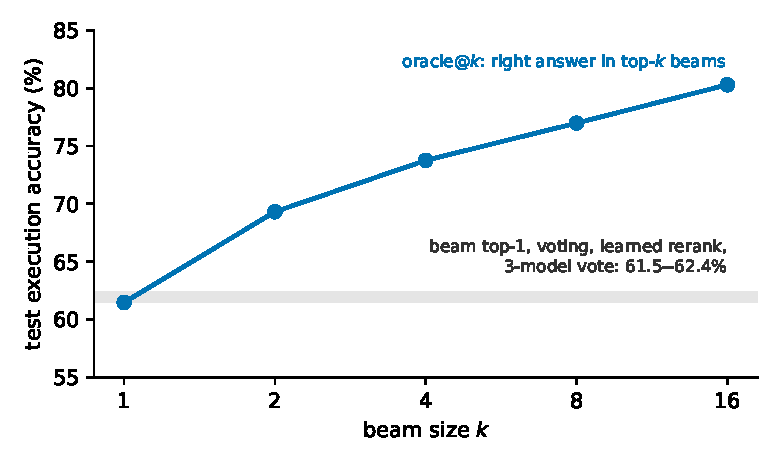
\includegraphics[width=0.7\textwidth]{figures/oracle_at_k.pdf}
\caption{The right answer is usually in the beam (oracle@$k$) but reranking recovers little of the gap.}\label{fig:oracle}
\end{figure}

By contrast, voting over independently trained models gains more: \VoteThree\% with three models and \VoteFour\% with four, against a single-model mean of \SingleEAMean\%, at the cost of training several models. Any of the three models contains the right answer for \AnyThree\% of questions. The candidates in one beam are therefore highly correlated: they tend to repeat the same mistake, so agreement among them is weak evidence of correctness. I did not test why (for example whether the early-stopping errors are shared by all beams), so this is a hypothesis, not a finding.

\section{Discussion, Limitations and Scope}

\paragraph{What the project shows.} (1) In this model family, retrieval quality is not what limits accuracy on FinQA: the released retriever misses evidence on hybrid questions, but a generator with full evidence is barely better. (2) The failures are in the program, and their form depends on length: premature stopping for multi-step programs, wrong operands and overlong programs for short ones. (3) The right program is often in the beam, but neither the model's probabilities nor agreement among beams finds it, and cheap reranking recovers about 0.4--0.6 points. A repair targeting the generator itself (for example length-aware training or decoding) is the natural next step, but I did not implement it.

\paragraph{Limitations.} All models use \code{roberta-base}, not the RoBERTa-large of the published number; \NRuns{} runs of one configuration give a rough variance estimate, not a confidence interval; the reranking gains are not statistically significant on 1{,}147 test questions; the oracle selector supplies gold facts plus the best non-gold facts up to $k$, so it measures the effect of complete evidence, not of removing all distractors; PA is lenient about constants (Sec.~\ref{sec:model}); the released retrieval has unknown provenance; and only FinQA was used. \emph{Not done:} the MultiHiertt generalization check from the plan, a retrieval-side repair, and larger encoders.

\section{Related Work}

FinQA and FinQANet \citep{chen2021finqa} define the task and the retriever--generator baseline that I reimplement. DyRRen \citep{li2023dyrren} adds a reranker that conditions on the partially generated program, and APOLLO \citep{sun2022apollo} improves retrieval and generation training objectives; both report accuracy gains but not a failure-mode breakdown. Reranking candidate programs by their execution results follows a general idea in neural program synthesis; here it is applied to FinQA and measured against an oracle. TAT-QA \citep{zhu2021tatqa}, ConvFinQA \citep{chen2022convfinqa} and MultiHiertt \citep{zhao2022multihiertt} are related hybrid-QA benchmarks.

\section{Code and Experiment Running Snippets}
Code: \todo{GitHub link}. The README lists every file, class and function, and which parts are my own: all of \code{src/}, \code{scripts/} and \code{tests/}. Only the FinQA data files and the pretrained RoBERTa weights are taken from outside. The released retriever rankings come from the FinQA release.
{\small
\begin{verbatim}
pip install -r requirements.txt
bash scripts/00_download_data.sh        # FinQA json files
python -m pytest -q                     # 68 tests
python scripts/01_validate_dsl.py       # gold programs re-execute

# CPU analyses (Tables 1-3, Fig. 1-3)
python scripts/01b_validate_preprocessing.py
python scripts/02_retrieval_analysis.py
python scripts/03_dataset_stats.py
python scripts/04_plot_retrieval.py

# GPU (Kaggle T4; notebooks/ has the exact runs)
python scripts/05_train_retriever.py --model roberta-base --out runs/retriever
python scripts/06_train_generator.py --model roberta-base \
       --retrieval released --seed 0 --out runs/gen_released
python scripts/07_taxonomy_report.py --pred runs/gen_released/pred_test.json \
       --oracle runs/gen_released/pred_test_oracle.json --name released

# Phase 2: beam search and reranking
python scripts/09_beam_decode.py --ckpt runs/gen_beam --beam 16      # GPU
python scripts/10_rerank_eval.py --beams runs/gen_beam --name released
python scripts/11_learned_rerank.py --beams runs/gen_beam --name released
python scripts/12_phase2_analysis.py     # error mechanisms, voting, figure
\end{verbatim}}

\bibliographystyle{plainnat}
\bibliography{references}

\end{document}
